
%%%%%%%%%%%%%%%%%%%%%%%%%%%%%%%%%%%%%%%%%%%%%%%%%%
\section{Elementary measure}
%%%%%%%%%%%%%%%%%%%%%%%%%%%%%%%%%%%%%%%%%%%%%%%%%%

\begin{reading}
  Tao, \S1.1.1
\end{reading}

In the introduction we saw that we cannot hope to define a measure which will work adequately on all subsets of $\RR^n$. In this section we start over and define a measure which is capable of measuring only the simplest sorts of subsets of $\RR^n$. In doing so we will see some of the difficulties which one encounters in defining even very simple measures, and we will also see some of these difficulties resolved. Moreover we will have explicit use for the elementary measure defined in this section, so doing so is not a digression at all.

Recall that a \emph{bounded interval} is any subset of $\RR$ of the form $(a,b)$, $[a,b)$, $(a,b]$, or $[a,b]$. We shall use the term \emph{box} for any subset of $\RR^n$ which is a Cartesian product of bounded intervals.

\begin{defn}
  A subset $E\subset\RR^n$ is \emph{elementary} if it can be expressed as a union of finitely many boxes.
\end{defn}

For any elementary set $E$, we wish to define its \emph{elementary measure}, or simply \emph{measure}, $m(E)$. The measure of any interval will be defined to be its length, and the measure of any box will be defined to be its volume. Thus if $I=(a,b)$ or $[a,b)$ or $(a,b]$ or $[a,b]$, then we let $m(I)=\len(I)=b-a$ (in all four cases). And if $B=\prod I_n$ is a box, then we define $m(B)=\vol(B)=\prod\len(I_n)$. Since we allow only bounded boxes, this product can never be indeterminate ($0\cdot\infty$). So far, so good.

We now wish to define the measure of an elementary set to be the sum of the finitely many boxes it is composed of. However there are two issues with this statement: first the constituent boxes need not be disjoint, and second there is in general more than one way to express an elementary set as a union of boxes. The following two lemmas address these two issues.

\begin{lem}
  Any elementary set $E$ can be expressed as a finite union of disjoint boxes.
\end{lem}

\begin{proof}
  First assume that $E\subset\RR^1$ and that $E=\bigcup I_i$. Then by considering all endpoints of the $I_i$ in increasing order $a_1,\ldots,a_m$ it is easy to write $E$ as the union of sets of the form $(a_i,a_{i+1})$ together with sets of the form $[a_i,a_i]$ (single points). Such a union is clearly disjoint.

  In general if $E\subset\RR^n$ and $E=\bigcup B_i$ then for each dimension $d\leq n$ consider in turn the $d$th sides of the boxes $I_i^d$. Again consider the endpoints of these intervals in increasing order $a_i^d,\ldots,a_{m_d}^d$. Then we can write $E$ as a union of small boxes which are products of sets of the form $(a_i^d,a_{i+1}^d)$ or of the form $[a_i^d,a_{i+1}^d]$. Such boxes are again disjoint.
\end{proof}

Figure~\ref{fig:elementary-disjoint} shows an example of the method of the proof above.

\begin{figure}[h]
  \centering
  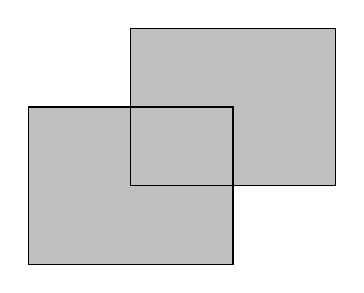
\begin{tikzpicture}[xscale=1.3]
    \draw[fill=gray!50] (0,0) rectangle (2,2);
    \draw[fill=gray!50] (1,1) rectangle (3,3);
    \draw (0,0) rectangle (2,2);
  \end{tikzpicture}
  \qquad
  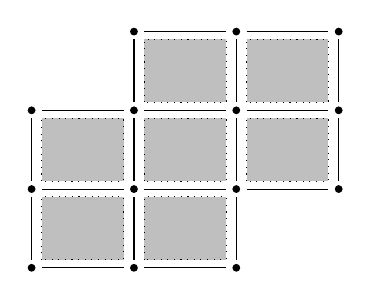
\begin{tikzpicture}[xscale=1.3]
    \draw[dotted,fill=gray!50] (.1,.1) rectangle (.9,.9);
    \draw[dotted,fill=gray!50] (1.1,.1) rectangle (1.9,.9);
    \draw[dotted,fill=gray!50] (.1,1.1) rectangle (.9,1.9);
    \draw[dotted,fill=gray!50] (1.1,1.1) rectangle (1.9,1.9);
    \draw[dotted,fill=gray!50] (2.1,1.1) rectangle (2.9,1.9);
    \draw[dotted,fill=gray!50] (2.1,2.1) rectangle (2.9,2.9);
    \draw[dotted,fill=gray!50] (1.1,2.1) rectangle (1.9,2.9);
    \draw (.1,0)--(.9,0);
    \draw (1.1,0)--(1.9,0);
    \draw (.1,1)--(.9,1);
    \draw (1.1,1)--(1.9,1);
    \draw (2.1,1)--(2.9,1);
    \draw (.1,2)--(.9,2);
    \draw (1.1,2)--(1.9,2);
    \draw (2.1,2)--(2.9,2);
    \draw (1.1,3)--(1.9,3);
    \draw (2.1,3)--(2.9,3);
    \draw (0,.1)--(0,.9);
    \draw (0,1.1)--(0,1.9);
    \draw (1,.1)--(1,.9);
    \draw (1,1.1)--(1,1.9);
    \draw (1,2.1)--(1,2.9);
    \draw (2,.1)--(2,.9);
    \draw (2,1.1)--(2,1.9);
    \draw (2,2.1)--(2,2.9);
    \draw (3,1.1)--(3,1.9);
    \draw (3,2.1)--(3,2.9);
    \node[circle,fill,inner sep=1pt] at (0,0) {};
    \node[circle,fill,inner sep=1pt] at (1,0) {};
    \node[circle,fill,inner sep=1pt] at (2,0) {};
    \node[circle,fill,inner sep=1pt] at (0,1) {};
    \node[circle,fill,inner sep=1pt] at (1,1) {};
    \node[circle,fill,inner sep=1pt] at (2,1) {};
    \node[circle,fill,inner sep=1pt] at (3,1) {};
    \node[circle,fill,inner sep=1pt] at (0,2) {};
    \node[circle,fill,inner sep=1pt] at (1,2) {};
    \node[circle,fill,inner sep=1pt] at (2,2) {};
    \node[circle,fill,inner sep=1pt] at (3,2) {};
    \node[circle,fill,inner sep=1pt] at (1,3) {};
    \node[circle,fill,inner sep=1pt] at (2,3) {};
    \node[circle,fill,inner sep=1pt] at (3,3) {};
  \end{tikzpicture}
  \caption{On the left: An elementary set which is a union of two closed boxes. On the right: the same elementary set expressed as a disjoint union of seven open boxes, 20 open segments, and 14 points.}
  \label{fig:elementary-disjoint}
\end{figure}

\begin{lem}
  Suppose the elementary set $E$ can be expressed in two ways a a finite union of disjoint boxes: $E=\bigsqcup B_i=\bigsqcup C_j$. Then $\sum\vol(B_i)=\sum\vol(C_j)$.
\end{lem}

\begin{proof}
  We first note that $I$ is an interval with endpoints $a,b$, and if $a=a_1,a_2,\ldots,a_m=b$ is an increasing sequence then $\len(I)=\sum\len(a_i,a_{i+1})$. This is simply because the latter summation telescopes.

  Next if $B$ is a box whose $d$th side has endpoints $a^d,b^d$, and if $a^d=a_1^d,a_2^d,\ldots,a_{m_d}^d=b^d$ then $\vol(B)=$ the sum of all small boxes of the form $\prod(a_{i_d}^d,a_{i_d+1}^d)$. We will call the set of such small boxes a perfect grid. Intuitively, if you break a box into a perfect grid of sub-boxes, then the volume of the box is the sum of the volumes of the sub-boxes.

  Now if $B$ is a box and one expresses it as a disjoint union of sub-boxes $B=\bigsqcup B_i$, then $\vol(B)=\sum\vol(B_i)$. This is because it is possible to find a \emph{refinement} of the given disjoint union which is a perfect grid as in the previous paragraph. That is, it is possible to write $B=\bigsqcup D_i$ where $\{D_i\}$ is a perfect grid, and each $B_i$ is the union of a perfect grid of sets taken from the collection $\{D_i\}$. Then one can simply apply the argument of the previous paragraph to $B$ and to each $B_i$.

  Finally given $E$, $B_i$, and $C_j$ as in the problem statement, one can find a third expression $E=\bigsqcup D_k$ where $\{D_k\}$ is a refinement of \emph{both} $\{B_i\}$ and of $\{C_j\}$. That is, each $B_i$ and each $C_j$ is a disjoint union of elements of $\{E_k\}$. It follows from the previous paragraph that $\sum\vol(B_i)=\sum\vol(D_k)$ and analogously that $\sum\vol(C_j)=\sum\vol(D_k)$. This completes the proof.
\end{proof}

The two lemmas together imply that it is well-defined to characterize the elementary measure with the expression $m(\bigsqcup B_i)=\sum m(B_i)$.

\begin{prop}
  The elementary measure function $m$ satisfies
  \begin{enumerate}
  \item (normality) $m(B)=\vol(B)$ for any box $B$;
  \item (translation-invariance) $m(x+E)=m(E)$ for any elementary set $E$; and
  \item (finite additivity) $m(E\cup F)=m(E)+m(F)$ for any disjoint elementary sets $E,F$.
  \end{enumerate}
\end{prop}

Normality is clear from the defenition of $m$. The translation-invarinace is easy because it is true of length and volume, and moreover is preserved even when we take disjoint unions. The finite additivity property is again clear from the definition of $m$. We remark that $m$ satisfies countable additivity as well (restricted to elementary sets of course), but that is much more difficult and will be addressed in the future.

The above three core properties imply further useful properties as well.

\begin{prop}
  \label{prop:elementary-further}
  The elementary measure function $m$ satisfies
  \begin{itemize}
  \item (monotonicity) $m(E)\leq m(F)$ for elementary sets $E\subset F$; and
  \item (finite subadditivity) $m(E\cup F)\leq m(E)+m(F)$ for elementary $E,F$.
  \end{itemize}
\end{prop}

These results give an essentially complete solution to the measure problem for elementary sets. It wasn't too difficult to achieve, but perhaps not as easy as one would have thought! Even so, what about measuring other simple sets such as circles, triangles, blobs, Cantor sets, and so on? In the next section we will continue on the road to doing this.

\begin{exerc}[Tao Ex 1.1.1]
  Show that the class of elementary sets is closed under the operations: union, intersection, set difference, symmetric difference, and translation.
\end{exerc}

\begin{exerc}
  Prove Proposition~\ref{prop:elementary-further}: The elementary measure satisfies the monotonicity and finite subadditivity properties.
\end{exerc}

\begin{exerc}[Tao Ex 1.1.4]
  Show that if $E$ is an elementary subset of $\RR^m$ and $F$ is an elementary subset of $\RR^n$ then $E\times F$ is an elementary subset of $\RR^{m+n}$. Furthermore show that $m_e(E\times F)=m_e(E)m_e(F)$.
\end{exerc}

\newpage